\documentclass[tikz]{standalone}
\usepackage{pgfplots}
\pgfplotsset{compat=1.15}
\usepackage{mathrsfs}
\usetikzlibrary{arrows,calc}
\usepackage{tkz-euclide}

\usepackage{fp}
\pagestyle{empty}

\definecolor{AngleClr}{rgb}{0,0.39215686274509803,0}
\definecolor{ShapeClr}{rgb}{0.6,0.2,0}

\definecolor{GreenShapeClr}{RGB}{60,138,32}
\definecolor{BlueShapeClr}{RGB}{22,115,168}

\begin{document}

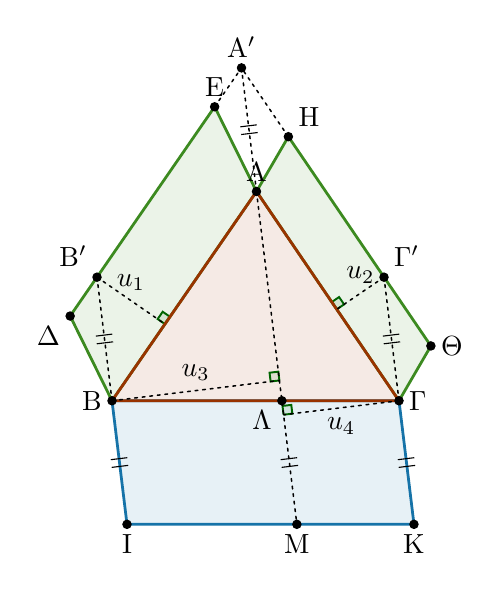
\begin{tikzpicture}[scale=.75]
\tkzSetUpLine[line width=1pt,color=black]
\tkzSetUpPoint[fill=black]

\def\Scale{1.35}
\FPeval{\Ax}{1.25 * \Scale}
\FPeval{\Ay}{3.6 * \Scale}
\FPeval{\Cx}{2.1 * \Ax}
\FPeval{\Ccx}{0.2 * \Scale}
\FPeval{\Cy}{1.45 * \Ax}
\FPeval{\Dx}{0.85 * \Ax}
\FPeval{\Dy}{(-1) * 0.42 * \Ax}
\FPeval{\Ty}{4 * \Scale}
\FPeval{\Tx}{0.55 * \Ax}

\tkzDefPoints{\Dy/\Dx/D,\Ay/0/C,\Cy/\Cx/B,0/0/A,\Ty/\Tx/Th}

\tkzDefParallelogram(B,A,D) \tkzGetPoint{E}
\tkzDefParallelogram(B,C,Th) \tkzGetPoint{H}

\tkzInterLL(D,E)(H,Th) \tkzGetPoint{A'}
\tkzDefPointWith[colinear= at A](A',B) \tkzGetPoint{I}
\tkzDefParallelogram(C,A,I) \tkzGetPoint{K}

\tkzInterLL(B,A')(A,C) \tkzGetPoint{L}
\tkzInterLL(B,A')(I,K) \tkzGetPoint{M}

\tkzFillPolygon[fill=ShapeClr,fill opacity=0.1](A,B,C)
\tkzFillPolygon[fill=GreenShapeClr,fill opacity=0.1](A,B,E,D)
\tkzFillPolygon[fill=GreenShapeClr,fill opacity=0.1](C,B,H,Th)
\tkzFillPolygon[fill=BlueShapeClr,fill opacity=0.1](A,C,K,I)

\tkzDefPointBy[symmetry=center A](I){}  \tkzGetPoint{B'}
\tkzDefPointBy[symmetry=center C](K){} \tkzGetPoint{C'}

\tkzDefPointBy[projection = onto B--L](A) \tkzGetPoint{BB}
\tkzDefPointBy[projection = onto B--L](C) \tkzGetPoint{CC}
\tkzDefPointBy[projection = onto A--B](B') \tkzGetPoint{BBB}
\tkzDefPointBy[projection = onto B--C](C') \tkzGetPoint{CCC}


\tkzMarkRightAngles[line width=0.7pt, size=.15,color=AngleClr,fill=AngleClr,fill opacity=0.1](B,BB,A B,CC,C B',BBB,B B,CCC,C')

\tkzDrawSegment[line width=0.55pt,color=black](A,D)
\tkzDrawSegments[line width=0.55pt,color=black,dashed,dash pattern=on 1pt off 1.75pt](B,M B',A C,C')

\tkzDrawPolygon[color=GreenShapeClr](A,B,E,D)
\tkzDrawPolygon[color=GreenShapeClr](C,B,H,Th)
\tkzDrawPolygon[color=BlueShapeClr](A,C,K,I)
\tkzDrawPolygon[color=ShapeClr](A,B,C)

\tkzDrawSegments[line width=0.55pt,color=black,dashed,dash pattern=on 1pt off 1.75pt](E,A' H,A' A',B A,BB C,CC B',BBB C',CCC)

\tkzDrawPoints[size=3](A,B,C,D,E,H,Th,A',I,K,L,M,B',C')
\tkzLabelPoint[left](A){$\rm B$}
\tkzLabelPoint[above](B){$\rm A$}
\tkzLabelPoint[right](C){$\rm \Gamma$}
\tkzLabelPoint[below left](D){$\rm \Delta$}
\tkzLabelPoint[above](E){$\rm E$}
\tkzLabelPoint[right](Th){$\rm \Theta$}
\tkzLabelPoint[above right](H){$\rm H$}
\tkzLabelPoint[above](A'){$\rm A'$}
\tkzLabelPoint[below](I){$\rm I$}
\tkzLabelPoint[below](K){$\rm K$}
\tkzLabelPoint[below left](L){$\rm \Lambda$}
\tkzLabelPoint[below](M){$\rm M$}
\tkzLabelPoint[above left](B'){$\rm B'$}
\tkzLabelPoint[above right](C'){$\rm \Gamma'$}

\tkzMarkSegments[mark=||,size=3](A',B A,I K,C L,M A,B' C,C')

\tkzLabelSegments[above](B',BBB){$u_1$}
\tkzLabelSegments[above](C',CCC){$u_2$}
\tkzLabelSegments[above](A,BB){$u_3$}
\tkzLabelSegments(C,CC){$u_4$}

\end{tikzpicture}

\end{document}
